% Chapter 1

\chapter{Introducción} % Chapter title

\label{ch:introduccion} % For referencing the chapter elsewhere, use \autoref{ch:introduccion} 
\lhead{\emph{Introducción}} % Change X to a consecutive number; this is for the header on each page - perhaps a shortened title

%----------------------------------------------------------------------------------------
Las antenas de arreglo de fase controlada son comunmente utilizadas en aplicaciones aéreas y espaciales. Para obtener un buen comportamiento 
de las mismas es necesario que estén correctamente calibradas. Esto implica, que las tolerancias de fases y amplitudes se mantengan y sus 
valores sean bien conocidas por cada elemento del arreglo.
 
Estas antenas en tierra son, generalmente, calibradas utilizando fuentes externas de campo lejano o cercano. Sin embargo, en aplicaciones 
aéreas o espaciales, la utilización de dichas fuentes son imprácticas o difícil de implementar. A su vez, si se opta por caracterizar todos
los componentes, el tiempo que implicaría es excesivo. Por estas razones, surgieron distintos métodos de calibración interna.

En este conexto, se propone un nuevo método de calibración, el cual aprovecha el acoplamiento mutuo inherente entre los módulos radiantes de
la antena.

La mayor parte de la energía eléctrica consumida hoy en día es generada por combustibles fósiles. Este hecho marca una clara situación
de dependencia de la economía mundial hacia estos recursos, causando inconvenientes como la excesiva
contaminación ambiental y su incipiente agotamiento, generando la necesidad de sustituirlos.

\section{DEFINICIÓN}
    
Una antena de arreglo de fase controlada es una antena compuesta por un conjunto de módulos radiantes dispuestos de tal forma, que, aplicando 
la teoría de construcción y desturcción de ondas, la señal emitida logra ser dirigida donde se desee.
    
Calibración interna es colocar sensores que permitan la medición directa u indirecta de la potencia y fase de salida/entrada de la antena 
polarimétrica.
    
\section{CARACTERÍSTICAS}
    
La utilización de una buena calibracíon interna es una problemática muy desafiante dado que es uno de los factores limitantes en la calidad de
los productos obtenidos con estas antenas.



Desde hace algún tiempo se ha estado gestando un gran interés por el desarrollo de las energías alternativas, motivado por la búsqueda
de fuentes eficientes, duraderas y poco contaminantes que podrían reemplazar las fuentes energéticas convencionales.
Dentro de ellas se cuentan principalmente la energía hidráulica, eólica y solar. Una de las desventajas de las mencionadas frente a los
combustibles es la posibilidad de ser almacenados para su disponibilidad inmediata. Sin embargo, existen también combustibles limpios,
como el \textbf{hidrógeno}.

El hidrógeno es un combustible de alto contenido energético y obtenible mediante diversos procesos, cuya reacción con el oxígeno produce agua
limpia. Estas características lo convierten en una opción atractiva frente al resto de los combustibles, tales como los hidrocarburos.

La utilización del hidrógeno como combustible para la generación de energía eléctrica se puede dar de varias maneras. Si bien su combustión
directa es una forma de obtener energía calórica que puede transformarse mediante procesos de conversión habituales, también puede conseguirse
energía eléctrica directamente usando mecanismos electroquímicos. Un modo de hacer esto es mediante \textbf{Celdas de combustible}.

\section{Celdas de combustible}
Las celdas de combustible son dispositivos electroquímicos que permiten obtener energía eléctrica a partir de la reacción química controlada
entre un combustible y un oxidante. Algunos de sus beneficios son su gran eficiencia comparada con las máquinas térmicas convencionales y
las reducidas emisiones de los procesos puestos en juego. Su utilización aún no es muy amplia debido a su elevado costo y la limitada
disponibilidad de los combustibles empleados.

Existen diversos tipos de celdas de combustible, aunque este trabajo solo se ocupa de las celdas de membrana de intercambio protónico
(PEM, por sus siglas en inglés), que operan a bajas temperaturas entregando potencia reducida. 

El uso práctico de las celdas comprende la disposición de varios elementos que forman un sistema. Por un lado, debido al reducido nivel
de tensión que entregan las celdas, suelen utilizarse arreglos de celdas en serie de modo que se obtenga un nivel adecuado de tensión entre
los electrodos terminales. Tales arreglos son llamados pilas de combustible. Por otro lado, durante la operación de las pilas se producen
fenómenos físicos, térmicos, electroquímicos, eléctricos, entre otros. Esto deriva en la necesidad de un sistema compuesto por un conjunto
de elementos auxiliares que tengan en cuenta los efectos de estos fenómenos sobre el comportamiento de la pila.

\section{Sistemas de generación híbridos}
Más allá de todas las ventajas mencionadas acerca de las celdas de combustible se han comentado varias de sus dificultades. La necesidad de
producir el combustible que consumen hace que pierdan autonomía. Es por ello que se ha sugerido su utilización en el contexto de los que se conocen 
como \textit{sistemas de generación híbrida} (SGH), cuyos módulos de generación extraen energía de diferentes fuentes. El presente trabajo 
se enmarca en el diseño de uno de estos sistemas, que en particular está compuesto por fuentes de energías limpias. En la fig. \ref{fig:sist_hibrido}
se muestra el esquema del sistema para el cual fue realizado este proyecto.

\begin{figure}[H]
 \centering
 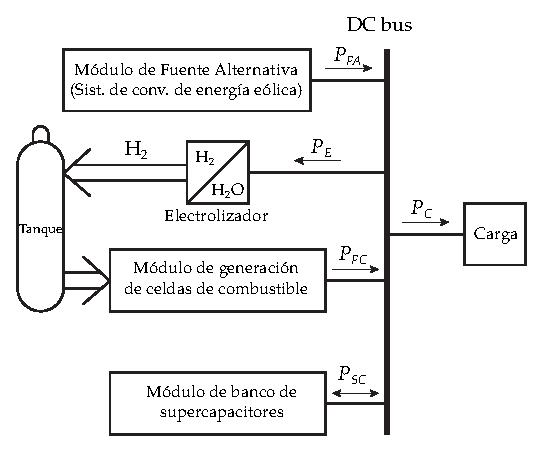
\includegraphics{gfx/diagrama_bloques_sistema_hibrido.eps}
 \caption{Diagrama en bloques de sistema híbrido}
 \label{fig:sist_hibrido}
\end{figure}

Para poder encarar la concepción del SGH se necesitarían todos los módulos que lo componen, esto representaría un gran costo. Por ello se ha
planteado una alternativa para el armado del sistema que consiste en la temporal sustitución de los módulos faltantes por plataformas de emulación.

\section{Emulador de pila de combustible}
El trabajo que se expone en el presente documento trata sobre el diseño y construcción de un emulador de pilas de combustible.
La necesidad del desarrollo de un emulador de pilas de combustible surge a partir de las diversas dificultades para obtener una pila
real, ya sea por su costo, su tamaño o el difícil acceso y almacenamiento del combustible.

La conexión de los módulos mostrados en la fig. \ref{fig:sist_hibrido} hacia el bus de tensión continua debe realizarse mediante una etapa de potencia 
que adapte los niveles eléctricos. En el proyecto del SGH, esta tarea ya ha sido abordada y constituyó el soporte para el desarrollo del emulador. 
La etapa de potencia consiste en un convertidor DC-DC conmutado elevador.

El flujo de trabajo del proyecto se llevó a cabo  de la siguiendo las tareas que se mencionan a continuación: en primer instancia se diseñaron los modelos
de simulación que luego fueron programados en el \emph{hardware} de control y se procedió a la realización de ciertos ajustes en la placa diseñada para el 
convertidor original cambiando la topología del mismo para permitirle funcionar según los modelos diseñados para finalmente realizar los ensayos finales.
